\documentclass[10pt]{beamer}

\usetheme{Frankfurt}

%%% Работа с русским языком
\usepackage{cmap}					% поиск в PDF
\usepackage{mathtext} 				% русские буквы в формулах
\usepackage[T2A]{fontenc}			% кодировка
\usepackage[utf8]{inputenc}			% кодировка исходного текста
\usepackage[english,russian]{babel}	% локализация и переносы
\usepackage{indentfirst}
\frenchspacing


%%% Дополнительная работа с математикой
\usepackage{amsmath,amsfonts,amssymb,amsthm,mathtools} % AMS
\usepackage{icomma} % "Умная" запятая: $0,2$ --- число, $0, 2$ --- перечисление

%% Номера формул
%\mathtoolsset{showonlyrefs=true} % Показывать номера только у тех формул, на которые есть \eqref{} в тексте.
%\usepackage{leqno} % Нумерация формул слева

%% Свои команды
\DeclareMathOperator{\sgn}{\mathop{sgn}}

%% Перенос знаков в формулах (по Львовскому)
\newcommand*{\hm}[1]{#1\nobreak\discretionary{}
	{\hbox{$\mathsurround=0pt #1$}}{}}

%%% Работа с картинками
\usepackage{graphicx}  % Для вставки рисунков
\graphicspath{{images/}}  % папки с картинками
\setlength\fboxsep{3pt} % Отступ рамки \fbox{} от рисунка
\setlength\fboxrule{1pt} % Толщина линий рамки \fbox{}
\usepackage{wrapfig} % Обтекание рисунков текстом
\usepackage{subfigure}

%%% Работа с таблицами
\usepackage{array,tabularx,tabulary,booktabs} % Дополнительная работа с таблицами
\usepackage{longtable}  % Длинные таблицы
\usepackage{multirow} % Слияние строк в таблице

%%% Программирование
\usepackage{etoolbox} % логические операторы

%
%\usepackage{fancyhdr} % Колонтитулы
% 	\pagestyle{fancy}
%\renewcommand{\headrulewidth}{0pt}  % Толщина линейки, отчеркивающей верхний колонтитул
% 	\lfoot{Нижний левый}
% 	\rfoot{Нижний правый}
% 	\rhead{Верхний правый}
% 	\chead{Верхний в центре}
% 	\lhead{Верхний левый}
%	\cfoot{Нижний в центре} % По умолчанию здесь номер страницы

\usepackage{setspace} % Интерлиньяж
%\onehalfspacing % Интерлиньяж 1.5
%\doublespacing % Интерлиньяж 2
%\singlespacing % Интерлиньяж 1

\usepackage{lastpage} % Узнать, сколько всего страниц в документе.

\usepackage{soul} % Модификаторы начертания


\usepackage{csquotes} % Еще инструменты для ссылок

%\usepackage[style=authoryear,maxcitenames=2,backend=biber,sorting=nty]{biblatex}

\usepackage{multicol} % Несколько колонок

\usepackage{tikz} % Работа с графикой
\usepackage{pgfplots}
\usepackage{pgfplotstable}

\renewcommand{\phi}{\varphi}
\renewcommand{\epsilon}{\varepsilon}
\usepackage[backend=biber, sorting=none]{biblatex}
\usepackage{subfigure}
\usepackage{authblk}

\addbibresource{lit.bib}

\theoremstyle{definition}
\newtheorem*{Def}{Определение}
\theoremstyle{plain}
\newtheorem{Lem}{Лемма}
\newtheorem{Th}{Теорема}

\newcommand{\delayV}[1]{\overset{\leftarrow}{\mathbf{x}}_{#1}}
\newcommand{\delayM}[1]{\overset{\leftarrow}{\mathbf{X}}_{#1}}

\title{Тензорная декомпозиция и прогноз для набора временных рядов}
%\author{Сёмкин Кирилл$^{1}$ \\ {\footnotesize $^{1}$semkin.ki@phystech.edu} \and Вадим Стрижов$^{2}$ \\ {\footnotesize %$^{2}$vadim.swifton@gmail.com}}

\author[1]{Сёмкин Кирилл}
\author[2]{Стрижов Вадим}

\affil[1]{{\footnotesize Московский физико-технический институт, semkin.ki@phystech.edu}}
\affil[2]{{\footnotesize strijov@ccas.ru}}

\date{}

\begin{document}
	
	\maketitle
	
	\begin{abstract}
		
		Обработка многомерных временных рядов связана с дополнительной сложностью моделирования связей между наблюдаемыми сигналами. Эти зависимости могут быть весьма существенными, и их игнорирование может привести к некорректным результатам анализа. В то же время их учёт делает модели сложнее, а решение связанных задач затруднительным. В данной работе предложен непараметрический метод, основанный на тензорном представлении многомерных сигналов и подходе SSA. Получен способ декомпозиции рядов, а также выведена формула и модель прогноза. Разработанная теория применяется к данным потребления электроэнергии и погоды, полученные результаты сравниваются с моделями mSSA, VAR, RNN.
		
	\end{abstract}
	
	\textbf{Ключевые слова}: {\small временные ряды, декомпозиция, прогноз, SSA, каноническое тензорное разложение}.
	
	
	\section{Введение}\label{Intro}
	
		Настоящая работа посвящена методам декомпозиции и построения прогноза для \textit{набора временных рядов} --- нескольких рассматриваемых вместе сигналов $ \{x_i(t)\}_{i=1}^m $, где $ t \in 1 \ldots N $. Нас будет интересовать аддитивная декомпозиция --- представление ряда в виде суммы нескольких составляющих.
		
		Методы разложения~\cite{enders2010applied, x11, cleveland90} и прогнозирования~\cite{3b1355aedd1041f1853e609a410576f3, enders2010applied, Box_Jenkins_methodology} для одиночного сигнала не могут быть просто перенесены на наборы временных рядов в случае их взаимной зависимости друг от друга. Для иллюстрации достаточно взять модель хищник-жертва \cite{Volterra:1928}. Размер популяции одних особей зависит от популяции других и наоборот. Мы будем предполагать некую связь входных рядов, строгое определение которой будет даваться в рамках рассматриваемых далее моделей. Выявление же этой связи --- отдельная задача, см., например,~\cite{702ab909-8cb1-3c30-a5f1-ab4517d6cf1c, 2012Sci...338..496S}.
		
		Рассмотрим несколько подходов, учитывающих фактор взаимозависимости. Модель \textit{рекуррентных нейронных сетей} (RNN) \cite{neco, TEALAB2018334} связывает ряды со своими предыдущими реализациями композицией однотипных нелинейных преобразований. На каждом шаге происходит вычисление скрытого представления, инкапсулирующего в себе информацию о прошлом и текущем состоянии сигналов. С его помощью строится предсказания будущих значений \cite{ZHANG2023143, HEWAMALAGE2021388}. 
		
		\textit{Векторная авторегрессия} (VAR)~\cite{VAR_model1, doi:10.1080/01621459.1962.10480664} представляет собой линейную стохастическую модель набора временных рядов. Если из значений сигналов в момент $ t $ составить вектор $ \mathbf{x}_t = (x_1(t) \ldots x_m(t))^{\mathsf{T}} $, то динамика имеет вид:
		
		\begin{equation*}
			\mathbf{x}_t = \boldsymbol{\mu} + \sum\limits_{i = 1}^p A_i \mathbf{x}_{t - i} + \mathbf{u}_t
		\end{equation*}
		
		Здесь $ \boldsymbol{\mu} $ - некоторый константный вектор, $ A_i $ матрицы $ m \times m $, $ \mathbf{u}_t $ - случайный вектор (например, реализация белого шума $ \text{WN}(t) $). Связь рядов задаётся линейными преобразованиями $ A_i $, т.е. каждый сигнал зависит как от собственных значений в прошлом, так и от прошлого других сигналов, \textit{линейным образом}. 	
		
		Рассмотренные решения позволяют строить прогноз, но имеют большое количество подбираемых гиперпараметров и требуют затратных процедур обучения. Более того, структура этих моделей не содержит способа построения декомпозиции временных рядов. 
		
		В связи с этим мы разработали новый метод \emph{tSSA}, имеющий всего две настраиваемых переменных и основывающийся на каноническом тензорном разложении CPD~\cite{kolda_tensors}. Его вычисление --- единственная необходимая процедура для получения декомпозиции и предсказания. Этот поход является расширением метода SSA(Гусеница)~\cite{ecfb9dc578be43ae9ee8fc88b8ff9151} для многомерных временных рядов и опирается на теорию динамических систем --- модель \textit{собственного пространства сигнала}~\cite{1572261550523548160}. Её суть состоит в построении фазового представления временных рядов (рис.\ref{pic:phase_traj}). 
		
		Существует и другая модификация Гусеницы --- mSSA~\cite{mSSA_overview}, отличающаяся от нашей в способе представления данных. Этот метод оперирует только двухиндексными объектами и их разложениями. Тем не менее они имеют общие идеи решения рассматриваемых задач, основанные на SSA.
		
		\begin{figure}[h]
			\centering
			\includegraphics[width=0.9\textwidth, keepaspectratio]{../figs/phase_traj.png}
			\caption{Пример построения фазовой траектории временного ряда}\label{pic:phase_traj}
		\end{figure}
		
		Далее в работе будет формально введена математическая модель порождения временных рядов, поставлена задача поиска базиса в пространстве сигналов и предложено её решение. На его основе будет рассмотрен наш способ построения декомпозиции и прогноза для рядов, а также проанализированы его свойства и вычислительные особенности. Далее, упомянутые методы будут применены к реальным данным потребления электроэнергии и погоды для получения прогноза и декомпозиции. Для последней будет введена специальная метрика; все результаты будут подкреплены иллюстрациями и выводами.
		 
	\section{Постановка задачи}\label{sec:problem_statement}
		 
		 Пусть имеется набор временных рядов $ \{x_i(t)\}_{i=1}^m $, порождённых некой \emph{динамической системой} $f$. Под этим понимается модель эволюции в дискретном времени обобщённых координат $ \mathbf{y} \in X $:
		 	
		 \begin{gather*}
		 	\mathbf{y}(t + 1) = f(\mathbf{y}(t)), \ t \in \mathbb{N} \\
		 	\mathbf{y}(0) = \mathbf{y}_0
		 \end{gather*}
		 	
		 В общем случае $ X $ --- гладкое многообразие большой размерности. Далее, каждая траектория этой системы порождает наблюдаемые ряды через неизвестное отображение $ \boldsymbol{\phi}: X \to \mathbb{R}^m $:
		 	
		 \begin{equation*}
		 	\boldsymbol{\phi}(\mathbf{y}(t)) = \mathbf{x}_t \Leftrightarrow \begin{cases}
		 		\phi_1(\mathbf{y}(t)) = x_1(t) \\
		 		\ldots \\
		 		\phi_m(\mathbf{y}(t)) = x_m(t) \\
		 	\end{cases}
		 \end{equation*}
		 	
		 Выдвигается предположение, что траектории $ \mathbf{y}(t) $ лежат в многообразии $ M \subset X $ размерности меньшей, чем у $ X $. Ставится задача поиска вложения (embedding) $ M $ в $ \mathbb{R}^{L} $ для некоторого $ L $ и нахождения базиса в образе этого вложения. С помощью него мы получим описание исходной системы в терминах стандартного линейного пространства, а значит и удобное описание наблюдаемых $ x_i(t) $.
		 
		 \subsection*{Случай единственного сигнала}
		 
		 	Предлагаемое нами решение существенно опирается на методику SSA и теорему Такенса~\cite{citeulike:2735031}. Кратко опишем их. Теорема формулируется для случая одного наблюдаемого сигнала и предъявляет явный вид вложения: произвольной точке $ \mathbf{y}(t) \in M $ ставится в соответствие вектор:
		 	
		 	 \[
		 	 	( \, \boldsymbol{\phi} \circ f^{t - L + 1}(\mathbf{y}(t)), \ldots , \boldsymbol{\phi} \circ f(\mathbf{y}(t)), \boldsymbol{\phi} \circ \mathbf{y}(t) \,)^{\mathsf{T}} = (x(t - L + 1), \ldots , x(t-1), x(t))^{\mathsf{T}}
		 	 \] 
		 	 
		 	Он называется \emph{вектором задержки} ряда в момент $ t $ и обозначается $ \delayV{t} $. Размерность таких векторов должна удовлетворять условию $ L > 2 \cdot \dim(M) $ , а функция $ \phi(\cdot) $ некоторым условиям регулярности, которые мы далее будем считаем выполненными.
		 	
		 	Т.о., имея временной ряд $ x(t) $ длины $ N $, получаем $ N - L + 1 $ векторов задержки. Построенное пространство вложения $ \text{Lin}(\{\delayV{t}\}) $, оно же \emph{собственное пространство сигнала} $ x(t) $, не должно иметь большую размерность, т.е. $ \text{Lin}(\{\delayV{t}\}) \subset \mathbb{R}^L $. Ортонормированный базис в этом пространстве выбирается как $ U $-компонента SVD-разложения матрицы векторов задержек --- так называемой \emph{траекторной матрицы} $ \mathbf{H}_x = [ \delayV{1} \ldots  \delayV{N - L + 1}] $.
		 	
		 \subsection*{Взаимосвязь рядов и метод tSSA}\label{sec:tssa_method}
		 
		 	Теперь обобщим данный подход на несколько временных рядов.
		 
		 	\begin{figure}[h]
		 		\centering
		 		\subfigure{\includegraphics[width=0.4\textwidth, keepaspectratio]{../figs/Trajectory_Tensor_1}}
		 		\subfigure{\includegraphics[width=0.4\textwidth, keepaspectratio]{../figs/Trajectory_Tensor_2}}
		 		
		 		\caption{Два вида на траекторный тензор. Слева --- в виде набора траекторных матриц сигналов $ \{x_i(t)\}_{i=1}^m $. Справа --- в виде набора матриц задержки.}\label{pic:traj_tensor}
		 	\end{figure}
	    
	    	В данном случае $ \boldsymbol{\phi}(\cdot) $ уже многомерное, а значит вместо вектора задержки одного сигнала необходимо рассматривать их набор для всех $ m $ сигналов в момент $ t $. Т.е. образами вложения будут служить \emph{матрицы задержки} $ ( \delayV{1_t} \ldots \delayV{m_t} ) := \delayM{t} $. А на смену траекторной матрице приходит \textit{траекторный тензор} $ \mathbf{T} $ набора сигналов. Он складывается из матриц задержки, выстроенных подряд по второму измерению тензора, рис. \ref{pic:traj_tensor} слева. Конструкция аналогичная построению $ \mathbf{H}_x $. Из неё следует важное свойство: $ \mathbf{T} $ можно рассматривать и как состыковку траекторных матриц $ \mathbf{H}_{x_i} $ вдоль третьего измерения, рис. \ref{pic:traj_tensor} справа.
	    	
	    	Проводя рассуждения, аналогичные случаю одного сигнала, мы получаем \emph{собственное пространство набора рядов} в виде линейной оболочки их матриц задержек. Но нам необходимо построить его для каждого сигнала отдельно.
	    	
	    	Выше мы обещали дать определение взаимосвязи рядов в рамках нашей модели. 
	    	
	    	\begin{Def}
	    		Мы называем набор временных рядов \emph{связанным}, если они имеют одинаковое для всех собственное пространство с единым базисом.
	    	\end{Def}
	    	
	    	Настало время построить эти пространство и базис. Заметим, что для этого достаточно разложить траекторные матрицы каждого сигнала по общему набору факторов. Применим \textit{CP-разложение} к траекторному тензору и рассмотрим его вид для каждого сечения по третьему измерению:
	    	
	    	\begin{equation}\label{eq:tSSA_decomp}
	    		\mathbf{T} = \sum\limits_{i = 1}^{r} \mathbf{a}_i \otimes \mathbf{b}_i \otimes \mathbf{c}_i \Leftrightarrow \begin{cases}
	    			\mathbf{H}_{x_1} = \sum\limits^{r} \boldsymbol{\sigma}_{x_1}(i) \cdot \mathbf{a}_i  \mathbf{b}_i^{\mathsf{T}}  \\
	    			\mathbf{H}_{x_2} = \sum\limits^{r} \boldsymbol{\sigma}_{x_2}(i) \cdot \mathbf{a}_i  \mathbf{b}_i^{\mathsf{T}} \\
	    			\ldots \\
	    			\mathbf{H}_{x_m} = \sum\limits^{r} \boldsymbol{\sigma}_{x_m}(i) \cdot \mathbf{a}_i  \mathbf{b}_i^{\mathsf{T}} 
	    		\end{cases}
	    	\end{equation}
	    
	    	Проанализируем полученное. Разложение определяется каноническим тензорным рангом $ r $ и набором векторов, которые удобно упаковать в матрицы: $ A = [\mathbf{a}_1 \ldots \mathbf{a}_r]; B = [\mathbf{b}_1 \ldots \mathbf{b}_r]; C = [\mathbf{c}_1 \ldots \mathbf{c}_r] $. Строку $ k $ матрицы $ C $ мы обозначаем $ \boldsymbol{\sigma}_{x_k} $. Она имеет аналогичный набору сингулярных чисел смысл, однако они могут быть и отрицательными.
	    	
	    	Из определения CPD как разложения вида (\ref{eq:tSSA_decomp}) c минимальным $ r $ следует, что матрицы $ A, B, C $ имеют полный ранг. Общим собственным пространством сигналов является $ \text{Lin}(\{\mathbf{a}_i\}) $ с единым базисом $ \{\mathbf{a}_i\}_{i = 1}^r $, не обязательно ортогональным. В постановке задачи мы предполагали, что размерность вложения не должна быть большой, т.е. должно выполняться $ r \ll L $.
	    	
	    	Наконец заметим, что \emph{строки} матриц $ \mathbf{H}_{x_k} $ также являются векторами задержек, но размерности $ N - L + 1 $, и в их терминах общим пространством сигналов будет $ \text{Lin}(\{\mathbf{b}_i\}) $. Т.о. наш подход обладает согласованностью относительно выбора $ \delayV{k_t} $, чего нет у метода mSSA.
	    	
	    	В данном разложении связь рядов определяют $ \boldsymbol{\sigma}_{x_k} $ : если для сигналов они имеют нулевые элементы в непересекающихся позициях, то общее собственное пространство представится прямой суммой подпространств индивидуальных рядов. В случае же полной взаимосвязи все представления сигналов лежат в общем пространстве.
	    	
	    \subsection*{Декомпозиция набора рядов}\label{sec:decomposition}
	    
	    	Теперь мы можем представить каждый сигнал суммой компонент по следующему принципу: \emph{декомпозиция траекторной матрицы $ \mathbf{H}_{x_k} $ определяет декомпозицию временного ряда $ x_k(t) $}. Эта методика лежит в основе метода SSA. Т.к. разложение у каждой матрицы своё, то и сигналы можно обрабатывать независимо.
	    	
	    	В данном подходе основным является свойство \emph{ганкелевости} траекторных матриц --- равенства элементов антидиагоналей. Каждому временному ряду длины $ N $ взаимнооднозначно сопоставляется ганкелева матрица размера $ L \times (N - L + 1) $.
	    	
	    	Алгоритм декомпозиции следующий: предполагается, что факторы разложения $ \mathbf{H}_{x_k} $ можно сгруппировать таким образом, что, сложив их в каждой группе, мы получим ганкелевы матрицы $ C_1, \ldots, C_s $. Это бы в точности соответствовало представлению $ x_k(t) $ в виде суммы $ s $ сигналов. На практике такая ситуация почти нереализуема (см.~\cite{ecfb9dc578be43ae9ee8fc88b8ff9151}), поэтому все $ C_i $ дополнительно \emph{ганкелизируют} --- усредняют каждую антидиагональ. Обозначим это оператором $ \text{Hankel}(\cdot) $. 
	    	
	    	Т.о. описанную процедуру можно представить выражением:
	    	
	    	\begin{multline}\label{eq:decomp_method_ideal}
	    		\underline{\mathbf{H}_{x_k}} \overset{1}{=} \sum\limits_{i = 1}^{r} \boldsymbol{\sigma}_{x_k}(i) \cdot \mathbf{a}_i  \mathbf{b}_i^{\mathsf{T}} \overset{2}{=} \sum\limits_{i \in \mathbb{I}_1} \boldsymbol{\sigma}_{x_k}(i) \cdot \mathbf{a}_i  \mathbf{b}_i^{\mathsf{T}} + \ldots + \sum\limits_{i \in \mathbb{I}_s} \boldsymbol{\sigma}_{x_k}(i) \cdot \mathbf{a}_i  \mathbf{b}_i^{\mathsf{T}} \overset{3}{=} \\ \overset{3}{=} C_1 + \ldots + C_s \overset{4}{=} \underline{\text{Hankel}(C_1) + \ldots + \text{Hankel}(C_s)}  \Leftrightarrow x_k(t) = c_1(t) + \ldots c_s(t)
	    	\end{multline}
	    	
	    	Здесь $ \mathbb{I}_1 \sqcup \ldots \sqcup \mathbb{I}_s = \{1, \ldots, r\} $ --- выбранные группы индексов. Четвёртое равенство нуждается в обосновании, для этого докажем простое свойство оператора ганкелизации:
	    	
	    	\begin{Lem}
	    		Оператор $ \text{Hankel}(\cdot) $ линейный.
	    	\end{Lem}
	    	
	    	\begin{proof}
	    		Возьмём две матрицы $ A $ и $ B $ одного размера и рассмотрим их элементы с одной антидиагонали $ a_1, \ldots, a_n $ и $ b_1, \ldots, b_n $. Тогда соответствующая антидиагональ в $ \text{Hankel}(A + B) $ равна $ \dfrac{1}{n} \sum\limits^n (a_i + b_i) = \dfrac{1}{n} \sum\limits^n a_i + \dfrac{1}{n} \sum\limits^n b_i $, т.е. равна сумме антидиагоналей матриц $ \text{Hankel}(A) $ и $ \text{Hankel}(B) $.
	    		
	    		Для произвольного скаляра $ \alpha $ также очевидно $ \dfrac{1}{n} \sum\limits^n \alpha \cdot a_i = \alpha \dfrac{1}{n} \sum\limits^n a_i $, из чего следует $ \text{Hankel}(\alpha A) = \alpha \text{Hankel}(A) $.
	    	\end{proof}
	    	
	    	Теперь учитывая, что $ \mathbf{H}_{x_k} $ --- ганкелева по построению, мы полностью обосновали тождественность переходов в (\ref{eq:decomp_method_ideal}) и корректность процедуры декомпозиции временного ряда для любой выбранной группировки.
	    	
	    \subsection*{Оптимальная декомпозиция и её сложность}\label{sec:optimal_decomp}
	    	
	    	Несмотря на корректность имеющегося алгоритма, хочется группировать факторы так, что каждая матрица $ C_i $ была как можно более "<ганкелевой">. Это соответствует сформулированному принципу о связи разложения матриц и сигналов, а также повышает интерпретируемость компонент. Опишем задачу формально и исследуем её.
	    	
	    	Рассмотрим первое равенство в (\ref{eq:decomp_method_ideal}), а также применим к нему оператор ганкелизации:
	    	
	    	\begin{equation*}
	    		\begin{cases*}
	    			\mathbf{H}_{x_k} = \sum\limits_{i = 1}^{r} \boldsymbol{\sigma}_{x_k}(i) \cdot \mathbf{a}_i  \mathbf{b}_i^{\mathsf{T}} \\
	    			\mathbf{H}_{x_k} = \sum\limits_{i = 1}^{r} Hankel(\boldsymbol{\sigma}_{x_k}(i) \cdot \mathbf{a}_i  \mathbf{b}_i^{\mathsf{T}})
	    		\end{cases*}
	    	\end{equation*}
	    	
	    	Ещё раз напомним, что $ \mathbf{H}_{x_k} $ ганкелева по построению. Вычтем из первого втрое и обозначим $ H_i = \boldsymbol{\sigma}_{x_k}(i) \cdot \mathbf{a}_i  \mathbf{b}_i^{\mathsf{T}} - Hankel(\boldsymbol{\sigma}_{x_k}(i) \cdot \mathbf{a}_i  \mathbf{b}_i^{\mathsf{T}}) $, что соответствует невязке между исходной матрицей и её ганкелизацией. Т.о. получим:
	    	
	    	\begin{equation}\label{eq:residuals_equation}
	    		H_1 + \ldots + H_r = 0 \Leftrightarrow H_r = - \sum\limits_{j = 1}^{r - 1} H_j
	    	\end{equation}
	    	
	    	Теперь группировка факторов и ганкелевость итоговых матриц $ C_i $ (см. предыдущий подраздел) становится равносильна следующему: $ \sum_{k \in \mathbb{I}_i} H_k = 0, \  \forall i \in 1, \ldots, s $. Т.е. матрицы невязок суммируются в ноль внутри каждой группы. Далее, несложно заметить, что если существует разложение на $ s $ групп, то к нему можно прийти, разделяя имеющиеся группы факторов на две последовательно. Поэтому остановимся на этой упрощённой задаче.
	    	
	    	Из (\ref{eq:residuals_equation}) видно, что все матрицы невязок уже суммируются в $ 0 $, т.е. группу для $ H_r $ можно определить, сгруппировав оставшиеся невязки. Введём для каждой из них переменную-индикатор $ \beta_j \in \{0, 1\} $, показывающую, к какой из двух групп относится невязка. 
	    	
	    	Итак, ещё раз перечислим все условия. $ H_i $ в одной группе суммируются в $ 0 $; также считаем, что все они ненулевые (иначе мы уже имеем искомую группировку), т.е. в группе должно быть хотя бы две невязки. Т.о. задача поиска группировки свелась к следующей:
	    	
	    	\begin{equation}
	    		\begin{cases*}
	    			\sum\limits_{j = 1}^{r - 1} \beta_j H_j = 0 \\
	    			\beta_j \in \{0, 1\}, \ \forall j \in 1, \ldots, r \\
	    			\sum\limits_{i = 1}^{r - 1} \beta_j \ge 2
	    		\end{cases*}
	    	\end{equation}
	    	
	    	Для придания задаче более знакомого вида, во-первых, векторизуем каждую $ H_i $, и соберём все эти векторы в одну матрицу $ \Lambda $, а также введём $ \boldsymbol{\beta} = (\beta_1 \ldots \beta_{r-1}) $. Вспомним, что на практике мы не ждём идеальной ситуации суммирования в $ 0 $ матриц невязок (ганкелевости $ C_i $, см. предыдущий подраздел), нам достаточно сделать сумму как можно более близкой к нулю. Это приводит нас к конечной формулировке:
	    	
	    	\begin{equation}\label{eq:decomp_search_final}
	    		\begin{cases*}
	    			\lVert \Lambda \boldsymbol{\beta} \rVert \to \underset{\boldsymbol{\beta}}{\min} \\
	    			\beta_j \in \{0, 1\}, \ \forall j \in 1, \ldots, r \\
	    			\sum\limits_{i = 1}^{r - 1} \beta_j \ge 2
	    		\end{cases*}
	    	\end{equation}
	    	
	    	Назовём решение этой системы \emph{оптимальной декомпозицией ряда}. Она представляет из себя задачу наименьших квадратов с целочисленными ограничениями (ILS), которая, как показано в \cite{van1981another}, является NP-сложной. Все проведённые рассуждения приведём в виде:
	    	
	    	\begin{Th}
	    		Оптимальная декомпозиция ряда, в смысле поиска группировки факторов разложения траекторной матрицы ряда, является NP-сложной задачей.
	    	\end{Th}
	    	
	    	Несмотря на полученный результат, существуют методы и эвристики для сведения ILS к эффективно вычислим задачам, см. \cite{Grafarend2022}.
	    	
	    	
	    \subsection*{Прогноз для набора рядов}\label{sec:tssa_forecast}
	     
	    	Получение предсказания нашей модели сводится к восстановлению компонент векторов задержек каждого входного ряда. Т.к. мы построили общий для всех сигналов базис $ \{\mathbf{a}_i\}_{i = 1}^r $, то каждый сигнал может обрабатываться независимо.
	    	
	    	Если бы $ \{\mathbf{a}_i\}_{i = 1}^r $ был ортогональным, то мы бы могли применить технику прогнозирования SSA \cite{ecfb9dc578be43ae9ee8fc88b8ff9151}. Мы не имеем такой гарантии, поэтому процедуру необходимо модифицировать.
	    	
	    	Рассмотрим входной ряд $ x(t) $ и построим для него прогноз на один шаг вперёд. Вектор задержки $ \delayV{N + 1} = (x(N - L) \ldots x(N + 1))^{\mathsf{T}} $, в котором последняя компонента неизвестна, лежит в пространстве $ \text{Lin}(\{\mathbf{a}_i\}) $. В терминах вводимой ранее матрицы $ A \in \mathbb{R}^{L \times r} $ полного ранга (см. раздел \hyperref[sec:tssa_method]{Взаимосвязь рядов и метод tSSA}) это записывается как:
	    	
	    	\begin{align}\label{eq:main_pred_for_A}
	    		\delayV{N + 1} = A \boldsymbol{\lambda} &\Leftrightarrow \begin{cases}
	    			\mathbf{x}_{kn} = A_{kn} \boldsymbol{\lambda}  \\
	    			x(N + 1) = \mathbf{a}_{pr}^{\mathsf{T}} \boldsymbol{\lambda}
	    		\end{cases}, \text{ где } \\
	    		A &= \left( \dfrac{A_{kn}}{\mathbf{a}_{pr}^{\mathsf{T}}} \right) \nonumber \\
	    		\delayV{N + 1} &= (\mathbf{x}_{kn} \  x(N + 1))^{\mathsf{T}} \nonumber
	    	\end{align}
	    	
	    	Здесь $ \boldsymbol{\lambda} \in \mathbb{R}^r $; вектор задержки и матрица представлены в блочном виде, разделяющим известную часть сигнала (known) и его будущее значение (predicted). Для построения прогноза необходимо определить $ \boldsymbol{\lambda} $. 
	    	
	    	Матрица имеющейся СЛАУ $ A_{kn} \in \mathbb{R}^{(L - 1) \times r} $ имеет ранг не менее $ r - 1 $, но мы предположим, что удаление одной строчки оставит ранг полным. Как показывает практика, это необременительное условие. Сама система, в силу предположения модели $ r \ll L $, является переопределённой. Значит её решение разумно искать только в смысле наименьших квадратов: $ \boldsymbol{\lambda} = (A_{kn}^T A_{kn})^{-1} A_{kn}^T \mathbf{x}_{kn} $. В итоге прогноз модели даётся:
	    	
	    	\begin{equation}\label{eq:tssa_pred}
	    		x(N + 1) = \mathbf{a}_{pr}^{\mathsf{T}} (A_{kn}^T A_{kn})^{-1} A_{kn}^T \mathbf{x}_{kn}
	    	\end{equation}
	    
	    	 Здесь $ \mathbf{a}_{pr}^{\mathsf{T}} (A_{kn}^T A_{kn})^{-1} A_{kn}^T = \mathbf{d}^{\mathsf{T}} $ --- вектор-строка, и, вычислив её единожды, можно последовательно строить предсказания на произвольный горизонт вперёд.
	    	 
	    	 Теперь перепишем (\ref{eq:tssa_pred}) в терминах $ x(t) $:
	    	 
	    	 \begin{equation*}\label{eq:autoregr}
	    	 	x(t) = \sum\limits_{i = 1}^{L - 1} d_i \cdot x(t - i)
	    	 \end{equation*}
	    	 
	    	 Это выражение приводит нас к окончательному выводу о характере прогноза:
	    	 
	    	 \begin{Th}
	    	 	Модель прогнозируемого методом tSSA ряда --- \textit{авторегрессионная} $ AR(L - 1) $. Поведение прогноза полностью определяется коэффициентами авторегрессии $ d_i $, найденными в (\ref{eq:tssa_pred}).
	    	 \end{Th}
	    
	\section{Вычислительный эксперимент}	
	
		\subsection*{Цели и постановка}
	
			В данном разделе мы рассмотрим применение метода tSSA для декомпозиции и прогноза нескольких многомерных временных рядов, а также сравним его с другими моделями, упомянутыми во введении: mSSA, VAR, RNN. Упомянем, что mSSA по теории и применению во многом схожа с нашим методом, с её помощью можно решать обе упомянутые задачи. Две другие модели способны только к предсказанию.
		
			Для измерения \textbf{качества декомпозиции} введём метрики:
			
			\begin{Def}
				\emph{Абсолютной ошибкой ганкелизации} матрицы M назовём 
				
				\[
					\text{AHE} = \lVert M - \text{Hankel}(M) \rVert_2
				\] 
				
			\end{Def}	
			
			\begin{Def}		
				
				\emph{Относительной ошибкой ганкелизации} матрицы M назовём 
				
				\[
				\text{RHE} = \frac{\text{AHE}}{\lVert M \rVert_2} 
				\] 		
				
			\end{Def}
			
			AHE можно представлять как суммарное стандартное отклонение антидиагоналей матрицы. RHE её более интерпретируемая модификация, которая и будет использоваться далее. 
			
			Напомним, что разложение ряда на компоненты эквивалентно группировке факторов разложения траекторной матрицы сигнала, т.е. получению матриц $ C_i $ (см. раздел \hyperref[sec:decomposition]{Декомпозиция набора рядов}). Именно для них мы и будем рассчитывать RHE, а также среднее RHE по одному ряду --- $ \overline{\text{RHE}}_{ts} $, и среднее RHE всех рядов датасета --- $ \overline{\text{RHE}} $.
			
			Для измерения \textbf{качества прогноза} ряда будем использовать стандартные метрики: среднеквадратическую ошибку $ \text{MSE}_{ts} $ и среднюю абсолютную процентную ошибку $ \text{MAPE}_{ts} $, а также их усреднения по всему датасету c обозначениями $ \overline{\text{MSE}} $ и $ \overline{\text{MAPE}} $.
			
			В качестве сигналов будут рассмотрены два набора данных: потребление электроэнергии и её цена за единицу мощности (рис. \ref{fig:electr_data}); а также три ряда, характеризующие погоду г. Берлин в период с 1980 по 1990 год: средние за день температура, осадки и атмосферное давление (рис. \ref{fig:weather_data}). Мы предполагаем наличие связи рядов в каждом наборе (на основе экономических/физических причин), т.к. это важное условие применения нашего метода (см. \hyperref[sec:tssa_method]{Взаимосвязь рядов и метод tSSA}). Каждый ряд имеет длину $ \approx 3 \cdot 10^3 $, из которых $ 20\% $ --- отложенная выборка для оценки качества прогноза.
			
			\begin{figure}[h]
				\centering
				\includegraphics[width=0.48\textwidth, keepaspectratio]{../figs/Electricity_Production}
				\includegraphics[width=0.48\textwidth, keepaspectratio]{../figs/Electricity_Price}
				\caption{Многомерный ряд потребления электричества и его цены за единицу мощности}\label{fig:electr_data}
			\end{figure}
			
			\begin{figure}[h]
				\centering
				\includegraphics[width=0.48\textwidth, keepaspectratio]{../figs/Temperature.png}
				\includegraphics[width=0.48\textwidth, keepaspectratio]{../figs/Precipitation.png}
				\includegraphics[width=0.48\textwidth, keepaspectratio]{../figs/Pressure.png}
				\caption{Многомерный ряд физических величин: температуры, осадков и давления, измеренных на метеостанции г. Берлин}\label{fig:weather_data}
			\end{figure}
			
			Опишем нюансы применения метода tSSA. Во-первых, вычисление канонического ранга тензора --- NP-трудная задача \cite{HASTAD1990644}, поэтому каждый раз ранг разложения будет указываться явно. Во-вторых, используемый алгоритм CP-разложения --- ALS \cite{kolda_tensors}, имеет ошибку аппроксимации, из-за чего возникает неточность разложения траекторных матриц. Относительные величины этих невязок будут указаны ниже. В-третьих, для поиска декомпозиции рядов будет решаться задача ILS (\ref{eq:decomp_search_final}), в которой матрица имеет высокую строковую размерность. Для ускорения мы сократим её до нескольких сотен, что всё ещё будет много больше размерности искомого вектора параметров. Используемый солвер --- SCIP \cite{BolusaniEtal2024ZR}.
			
			Наконец, мы зафиксируем единый для всех моделей параметр, отвечающий за длину предуславливания методов на историю рядов, который обозначался за $ L $. Для tSSA и mSSA он был описан в начале раздела \ref{sec:problem_statement}; в RNN это можно считать длиной энкодера; в VAR это максимальная длина истории ряда, на которую производится авторегрессия. Везде ниже $ L = 500 $.		
				
		\subsection*{Результаты и обсуждение}
		
			Начнём с задачи прогнозирования. На рис. \ref{fig:mse_mape_electr} и \ref{fig:mse_mape_weather} отображена зависимость метрик качества прогноза tSSA в зависимости от ранга CP-разложения. Точка минимума и характер изменения MSE и MAPE совпадают. Наблюдается эффект переобучения при повышении значения ранга, особенно резкое ухудшение метрик у данных погоды. При этом ошибка CP-разложения монотонно убывает, см. рис. \ref{fig:cpd_errors}.
			
			\begin{figure}[h]
				\centering
				\includegraphics[width=0.48\textwidth, keepaspectratio]{../experiments/electricity/tssa/figs/prediction/MSE_rank.png}
				\includegraphics[width=0.48\textwidth, keepaspectratio]{../experiments/electricity/tssa/figs/prediction/MAPE_rank.png}
				\caption{Значения метрик $ \overline{\text{MSE}} $ и $ \overline{\text{MAPE}} $ предсказания tSSA для разных рангов CP-разложения. Отдельно выделен оптимальный ранг. Данные электроэнергии.}\label{fig:mse_mape_electr}
			\end{figure}
			
			\begin{figure}[h]
				\centering
				\includegraphics[width=0.48\textwidth, keepaspectratio]{../experiments/weather/tssa/figs/prediction/MSE_rank.png}
				\includegraphics[width=0.48\textwidth, keepaspectratio]{../experiments/weather/tssa/figs/prediction/MAPE_rank.png}
				\caption{Значения метрик $ \overline{\text{MSE}} $ и $ \overline{\text{MAPE}} $ предсказания tSSA для разных рангов CP-разложения. Отдельно выделен оптимальный ранг. Данные погодных условий.}\label{fig:mse_mape_weather}
			\end{figure}
			
			\begin{figure}[h]
				\centering
				\includegraphics[width=0.48\textwidth, keepaspectratio]{../experiments/electricity/tssa/figs/CPD_error.png}
				\includegraphics[width=0.48\textwidth, keepaspectratio]{../experiments/weather/tssa/figs/CPD_error.png}
				\caption{Относительные ошибки CPD-аппроксимации траекторных тензоров в зависимости от ранга разложения. Слева --- электроэнергии, справа --- погоды.}\label{fig:cpd_errors}
			\end{figure}
			
			Графики наилучшего прогноза tSSA приведены на рис. \ref{fig:tssa_electr_pred} и \ref{fig:tssa_weather_pred}, где наглядно видны различия метода с малым и большим рангом. В первом случае авторегрессионная модель прогноза большего порядка (см. теорему раздела \hyperref[sec:tssa_forecast]{Прогноз для набора рядов}), что позволяет точно аппроксимировать ряд. В случае же погоды большой порядок приводил к нестабильности и неограниченному росту, но при уменьшении степеней свободы возможно аппроксимировать сигналы только в среднем.
			
			Итоговые метрики качества прогноза всех моделей --- в табл. \ref{tab:pred_res_electr} и \ref{tab:pred_res_weather}. Наш метод показал наилучшие результаты, хотя mSSA был близок по точности. Метод VAR оказался нестабилен на выбранном горизонте прогнозирования, а RNN обучался в константную функцию.
			
			\begin{figure}[h]
				\centering
				\includegraphics[width=0.48\textwidth, keepaspectratio]{../experiments/electricity/tssa/figs/prediction/cpd_rank_30/Production_program.png}
				\includegraphics[width=0.48\textwidth, keepaspectratio]{../experiments/electricity/tssa/figs/prediction/cpd_rank_30/Price.png}
				\caption{Предсказание данных электроэнергии методом tSSA. CPD-ранг $ = 30 $}\label{fig:tssa_electr_pred}
			\end{figure}
			
			\begin{figure}[h]
				\centering
				\includegraphics[width=0.48\textwidth, keepaspectratio]{../experiments/weather/tssa/figs/prediction/cpd_rank_5/Temperature.png}
				\includegraphics[width=0.48\textwidth, keepaspectratio]{../experiments/weather/tssa/figs/prediction/cpd_rank_5/Precipitation.png}
				\includegraphics[width=0.48\textwidth, keepaspectratio]{../experiments/weather/tssa/figs/prediction/cpd_rank_5/Pressure.png}
				\caption{Предсказание данных погоды методом tSSA. CPD-ранг $ = 5 $}\label{fig:tssa_weather_pred}
			\end{figure}
			
			\def\arraystretch{1.1}
			\begin{table}[h]
				\centering
				\caption{Метрики моделей на прогнозировании данных электроэнергии}\label{tab:pred_res_electr}
				\begin{tabular}{|c|c|c|c|c|}
					\hline
					& \textit{tSSA}  & \textit{mSSA} & \textit{VAR} & \textit{RNN} \\ \hline
					$ \overline{\text{MSE}}_{\text{Producution}} $, $10^6$ & 1.24           & 1.51          & 7.81         & 2.70         \\ \hline
					$ \overline{\text{MSE}}_{\text{Price}} $, $10^3$      & 0.88           & 1.03          & 4.85         & 30.0         \\ \hline
					$ \overline{\text{MSE}} $, $10^6$             & \textbf{0.62}  & 0.75          & 3.91         & 135.00       \\ \hline
					$ \overline{\text{MAPE}}_{\text{Producution}} $        & 0.054          & 0.060         & 0.137        & 0.999        \\ \hline
					$ \overline{\text{MAPE}}_{\text{Price}} $             & 0.164          & 0.170         & 0.360        & 1.004        \\ \hline
					$ \overline{\text{MAPE}} $                    & \textbf{0.109} & 0.115         & 0.249        & 1.002        \\ \hline
				\end{tabular}
			\end{table}
			
			\def\arraystretch{1.1}
			\begin{table}[h]
				\centering
				\caption{Метрики моделей на прогнозировании данных погоды}\label{tab:pred_res_weather}
				\begin{tabular}{|c|c|c|c|c|}
					\hline
					& \textit{tSSA}                & \textit{mSSA} & \textit{VAR} & \textit{RNN} \\ \hline
					$ \overline{\text{MSE}}_{\text{Temp}} $  & 14.16                        & 20.12         & 40.67        & 177.84            \\ \hline
					$ \overline{\text{MSE}}_{\text{Prec}} $  & 11.02                        & 11.23         & 22.84        & 14.05            \\ \hline
					$ \overline{\text{MSE}}_{\text{Pres}} $  & 98.02                        & 101.23        & 156.75       & $ > 10^6 $            \\ \hline
					$ \overline{\text{MSE}} $        & \textbf{41.067}              & 44.193        & 73.420       & $> 3 \cdot 10^5$            \\ \hline
					$ \overline{\text{MAPE}}_{\text{Temp}} $ & 0.850 & 0.626         & 0.468        & 1.193            \\ \hline
					$ \overline{\text{MAPE}}_{\text{Prec}} $ & 3.151 & 2.834         & 4.637        & 2.026            \\ \hline
					$ \overline{\text{MAPE}}_{\text{Pres}} $ & 0.007 & 1.254         & 3.983        & 1.000            \\ \hline
					$ \overline{\text{MAPE}} $       & \textbf{1.336}               & 1.571         & 3.029        & 1.406            \\ \hline
				\end{tabular}
			\end{table}
			
			Теперь рассмотрим задачу декомпозиции. На рис. \ref{fig:decomp_rhe_rank} представлены зависимости качества разложения от значения CP-ранга. В обоих случаях $ \overline{\text{RHE}} $ достаточно быстро достигает минимума, после чего не меняется или растёт. Вспоминая аналогичный результат для прогнозирования, можно сделать вывод, что метод tSSA достигает наибольшей обобщающей способности на небольших канонических рангах траекторных тензоров данных. В свою очередь, этот ранг пропорционален размерности собственного пространства сигналов (см. начало раздела \ref{sec:problem_statement}). Из этого заключаем о выполнении главной теоретической предпосылки для применения нашего метода.
			
			На рис. \ref{fig:electr_decomp_tssa} и \ref{fig:weather_decomp_tssa} представлены результаты наилучшей найденной декомпозиции рядов на две компоненты методом tSSA. В силу вычислительной сложности задачи ILS, разложение на б$\acute{\text{о}}$льшее количество компонент не производится. Из графиков видно, как сильно общий базис сигналов влияет на их декомпозицию: для генерации электроэнергии и её цены компоненты получились почти идентичными, с точностью до смещения и масштаба. Аналогичная ситуация для температуры и осадков в данных погоды, а для атмосферного давления разложение получилось другим. Далее, на рис. \ref{fig:weather_decomp_tssa} метод выделил для каждого сигнала по две периодические составляющие: одна из них большой амплитуды, другая много меньшей. Небольшой шум остался в каждой компоненте. На рис. \ref{fig:electr_decomp_tssa} метод выделил по два высокочастотных колебания разной амплитуды и смещения.
			
			Для сравнения на рис. \ref{fig:electr_decomp_mssa} и \ref{fig:weather_decomp_mssa} приведены результаты декомпозиции методом mSSA на пять компонент. Для их получения не было необходимости в решении ILS или настраивания CP-ранка, но они подбиралась вручную на основе близости сингулярных чисел некоторой матрицы, см. \cite{ecfb9dc578be43ae9ee8fc88b8ff9151}. Тем не менее компоненты получились более интерпретируемыми и подробными: метод выделил несколько трендов и гармоник. Также, как видно из табл. \ref{tab:decomp_electr_results} и \ref{tab:decomp_weather_results}, mSSA немного выиграл по точности. Т.о. вычислительная сложность декомпозиции tSSA является главной проблемой метода и требует разработки собственных эвристик, которые, к слову, у mSSA уже имеются \cite{ecfb9dc578be43ae9ee8fc88b8ff9151}.		
			
		\section{Заключение}
		
		Тензорный метод tSSA был разработан для прогноза и декомпозиции набора временных рядов, обработка которых требует учёта фактора взаимосвязанности. Его главное достоинство --- проста в использовании: имеется всего два настраиваемых параметра, для которых не требуется изощрённых процедур обучения. Между тем, теория метода опирается на весьма общую модель динамических систем и предъявляет к данным лишь возможность маломерного представления. При применении на реальных датасетах удалось установить справедливость теоретических требований алгоритма, а также показать качество выше нейросетевых и статистических подходов. Главным вызовом для tSSA является результат о NP-сложности поиска оптимальной декомпозиции рядов. Нахождение способов решения этой проблемы или поиск другого пути для построения разложения --- основные направления дальнейшего развития метода.
		
		\begin{figure}[h!]
			\centering
			\includegraphics[width=0.48\textwidth, keepaspectratio]{../experiments/electricity/tssa/figs/decomposition/RHE_mean.png}
			\includegraphics[width=0.48\textwidth, keepaspectratio]{../experiments/weather/tssa/figs/decomposition/RHE_mean.png}
			\caption{Зависимость метрики $ \overline{\text{RHE}} $ от ранга CP-разложения. Слева --- для данных электроэнергии, справа --- погоды. Отдельно выделен оптимальный ранг.}\label{fig:decomp_rhe_rank}
		\end{figure}
		
		\begin{figure}[h!]
			\centering
			\includegraphics[width=0.48\textwidth, keepaspectratio]{../experiments/electricity/tssa/figs/decomposition/cpd_rank_20/Production_program.png}
			\includegraphics[width=0.48\textwidth, keepaspectratio]{../experiments/electricity/tssa/figs/decomposition/cpd_rank_20/Price.png}
			\caption{Разложение рядов на две компоненты методом tSSA. Данные электроэнергии. CPD-ранг $ = 20 $}\label{fig:electr_decomp_tssa}
		\end{figure}
		
		\begin{figure}[h!]
			\centering
			\includegraphics[width=0.48\textwidth, keepaspectratio]{../experiments/weather/tssa/figs/decomposition/cpd_rank_20/Temperature.png}
			\includegraphics[width=0.48\textwidth, keepaspectratio]{../experiments/weather/tssa/figs/decomposition/cpd_rank_20/Precipitation.png}
			\includegraphics[width=0.48\textwidth, keepaspectratio]{../experiments/weather/tssa/figs/decomposition/cpd_rank_20/Pressure.png}
			\caption{Разложение рядов на две компоненты методом tSSA. Данные погоды. CPD-ранг $ = 20 $}\label{fig:weather_decomp_tssa}
		\end{figure}
		
		
		\begin{figure}[h!]
			\centering
			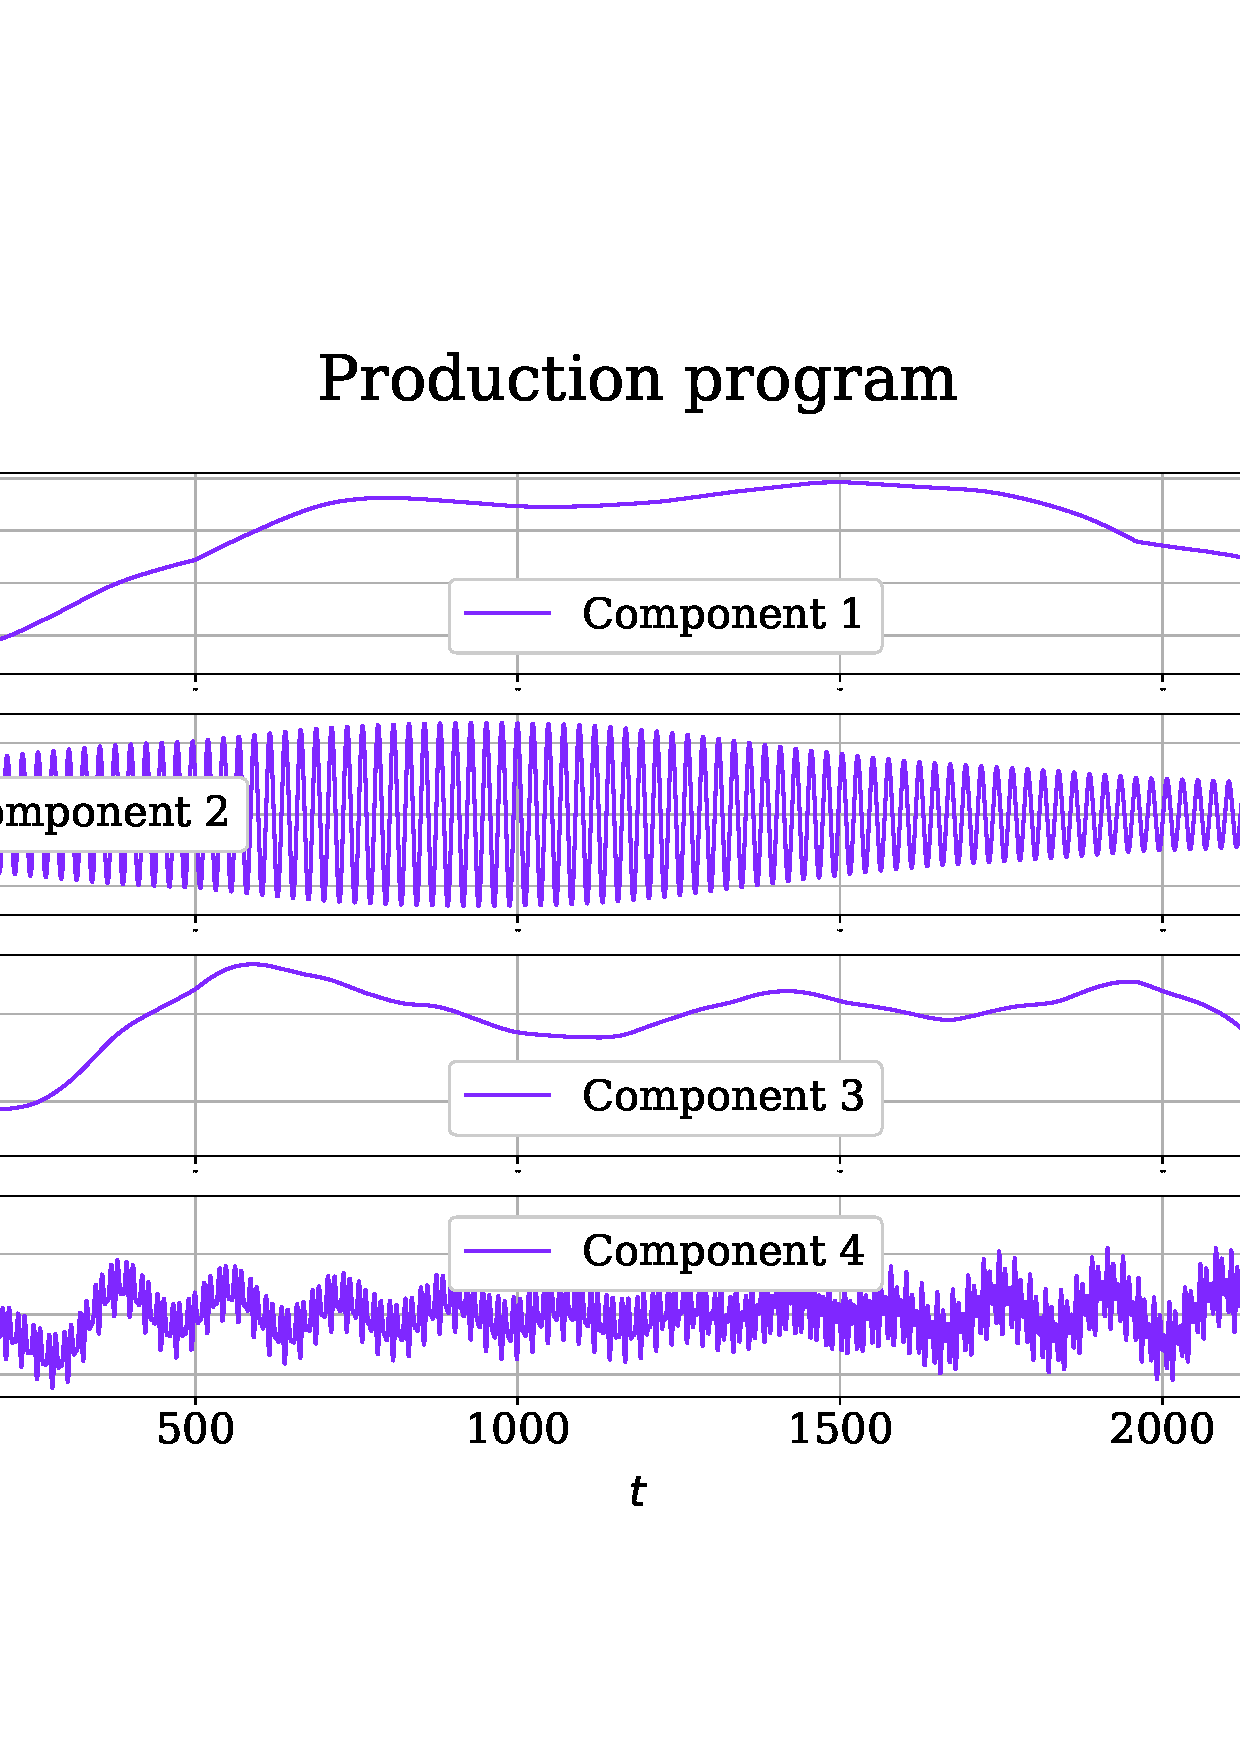
\includegraphics[width=0.48\textwidth, keepaspectratio]{../experiments/electricity/mssa/figs/decomposition/manual/grouping_1/Production_program.png}
			\includegraphics[width=0.48\textwidth, keepaspectratio]{../experiments/electricity/mssa/figs/decomposition/manual/grouping_1/Price.png}
			\caption{Разложение рядов на компоненты методом mSSA. Данные электроэнергии.}\label{fig:electr_decomp_mssa}
		\end{figure}
		
		\begin{figure}[h!]
			\centering
			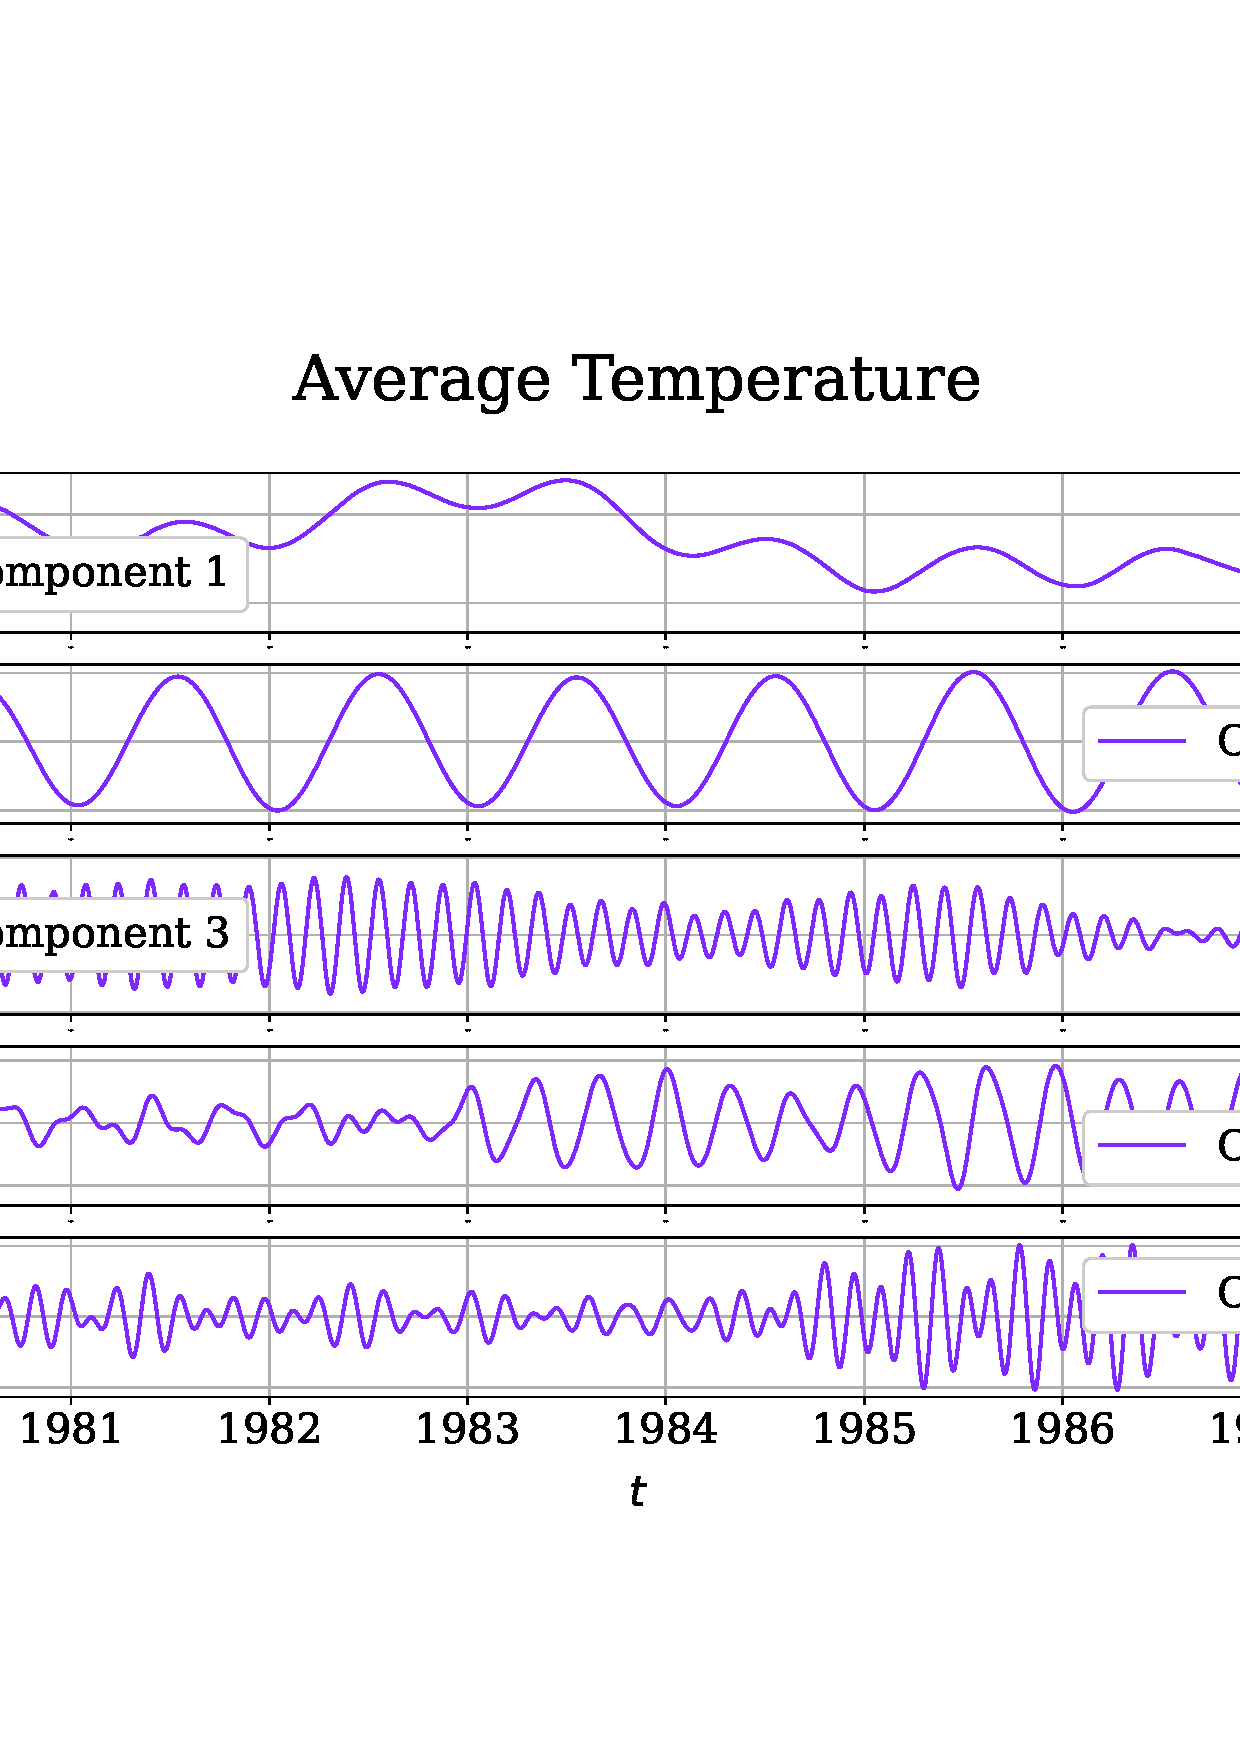
\includegraphics[width=0.48\textwidth, keepaspectratio]{../experiments/weather/mssa/figs/decomposition/manual/grouping_1/Average_Temperature.png}
			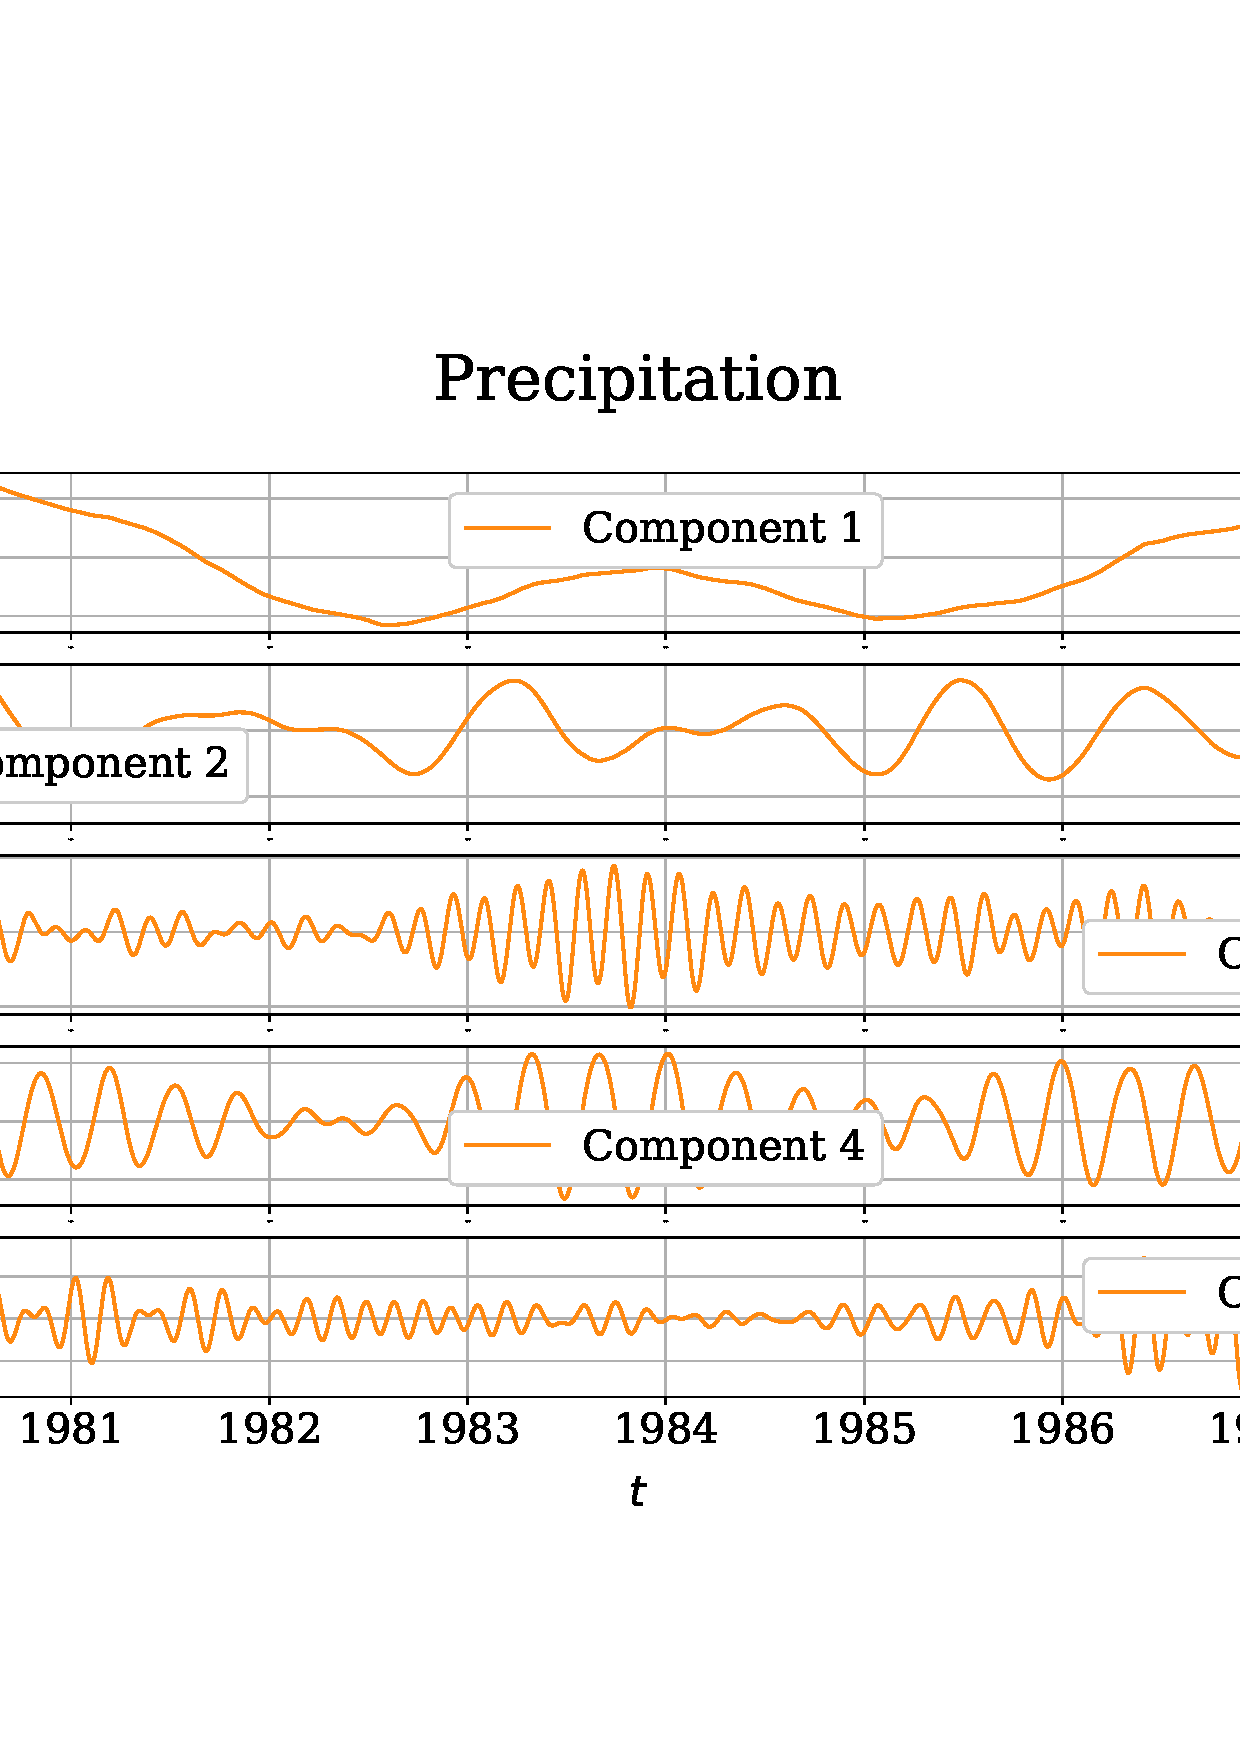
\includegraphics[width=0.48\textwidth, keepaspectratio]{../experiments/weather/mssa/figs/decomposition/manual/grouping_1/Precipitation.png}
			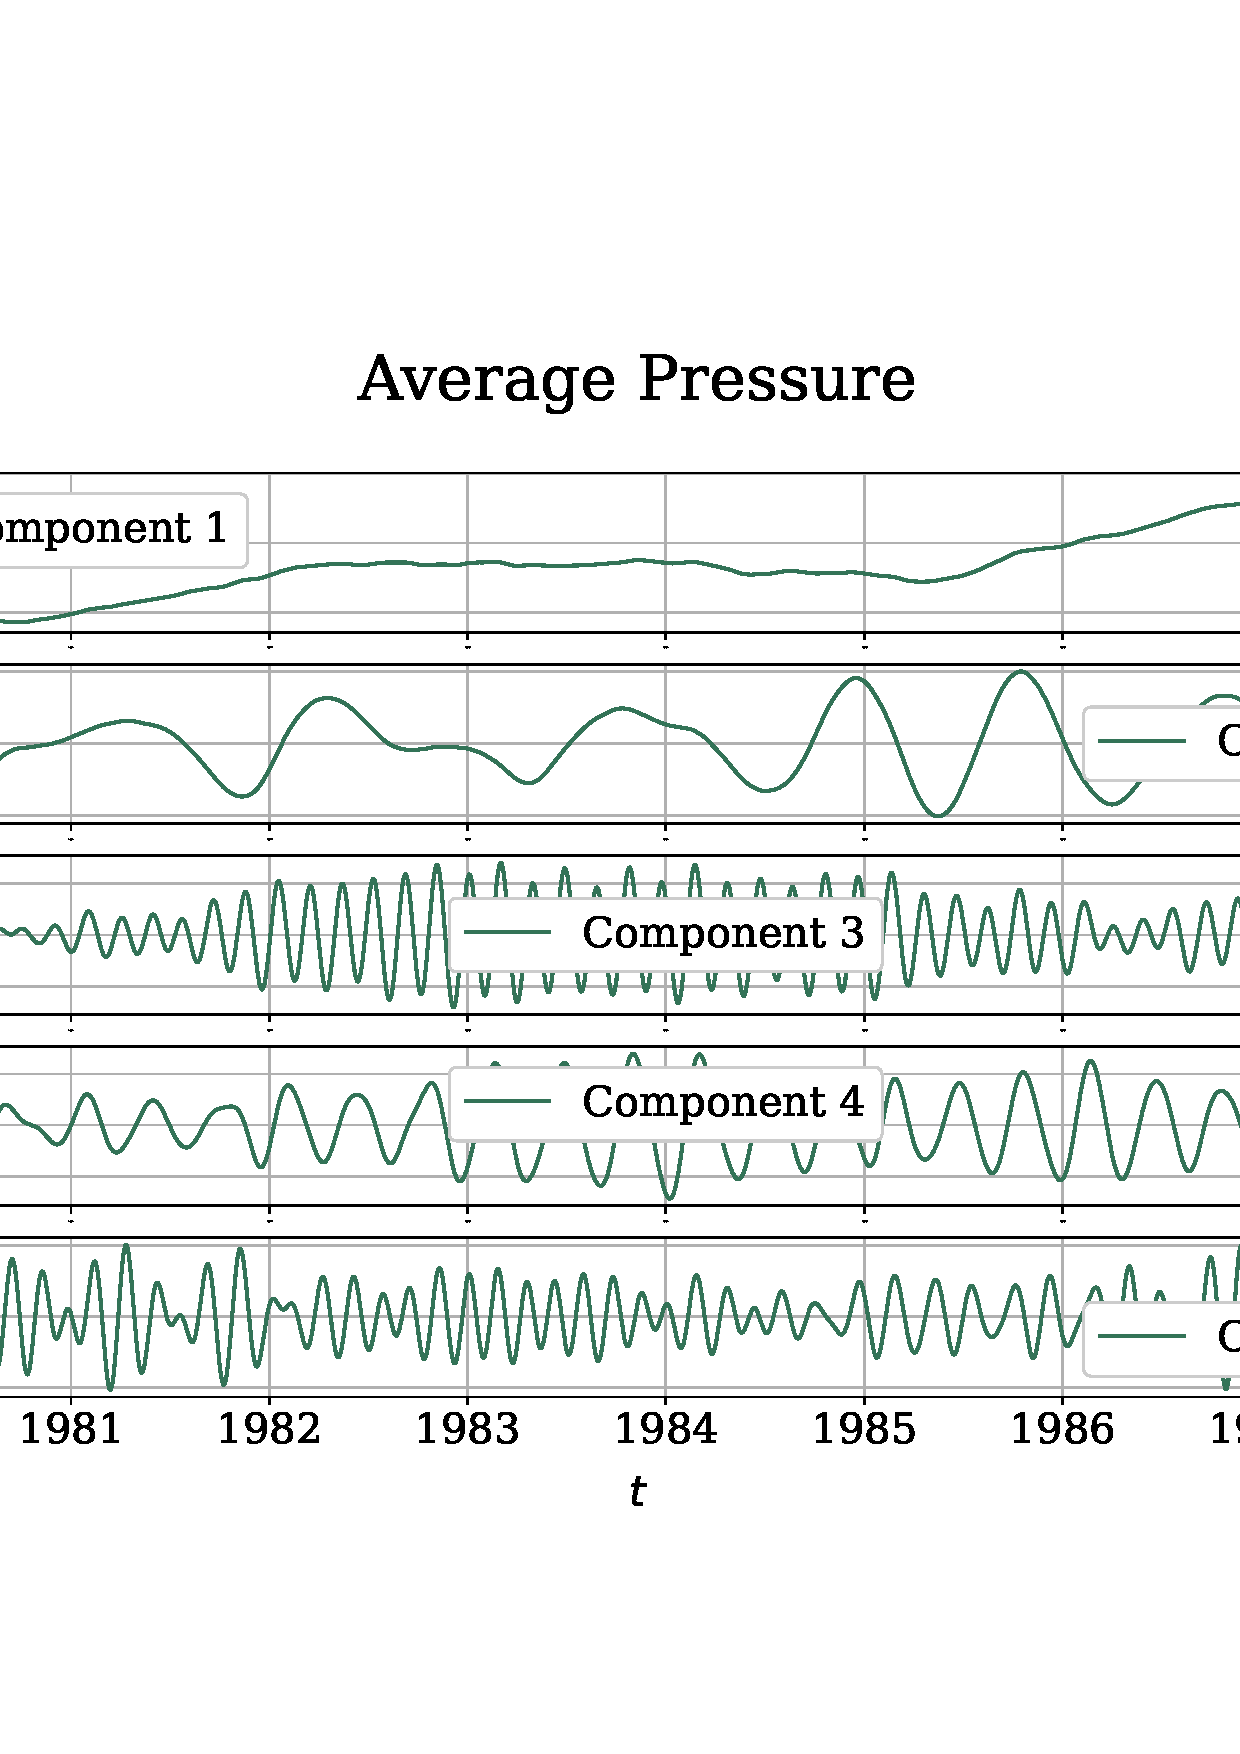
\includegraphics[width=0.48\textwidth, keepaspectratio]{../experiments/weather/mssa/figs/decomposition/manual/grouping_1/Average_Pressure.png}
			\caption{Разложение рядов на компоненты методом mSSA. Данные погоды.}\label{fig:weather_decomp_mssa}
		\end{figure}
		
		\def\arraystretch{1.2}
		\begin{table}[h!]
			\centering
			\caption{Метрики моделей на декомпозиции данных электроэнергии}\label{tab:decomp_electr_results}
			\begin{tabular}{|c|c|c|}
				\hline
				& tSSA  & mSSA           \\ \hline
				$ \overline{\text{RHE}}_{\text{Producution}} $  & 0.507 & 0.308          \\ \hline
				$ \overline{\text{RHE}}_{\text{Price}} $      & 0.511 & 0.31           \\ \hline
				$ \overline{\text{RHE}} $             & 0.509 & \textbf{0.309} \\ \hline
			\end{tabular}
		\end{table}
		
		\def\arraystretch{1.2}
		\begin{table}[h!]
			\centering
			\caption{Метрики моделей на декомпозиции данных погоды}\label{tab:decomp_weather_results}
			\begin{tabular}{|c|c|c|}
				\hline
				& tSSA  & mSSA           \\ \hline
				$ \overline{\text{RHE}}_{\text{Temp}} $   & 0.512 & 0.467          \\ \hline
				$ \overline{\text{RHE}}_{\text{Prec}} $ & 0.508 & 0.538          \\ \hline
				$ \overline{\text{RHE}}_{\text{Pres}} $   & 0.542 & 0.502          \\ \hline
				$ \overline{\text{RHE}} $         & 0.521 & \textbf{0.502} \\ \hline
			\end{tabular}
		\end{table}
			
		
		\clearpage
		\printbibliography
	
\end{document}